% \documentclass[9pt, compress, xcolor=table]{beamer}


% \usetheme{m}

% \usepackage{amsmath,amssymb,amsthm}
% \usepackage{latexsym}
% \usepackage{booktabs}
% \usepackage[scale=2]{ccicons}
% \usepackage{minted}
% \usepackage[english, russian]{babel}
% \usepackage{graphicx}
% \usepackage{xcolor}
% \usepackage{tabu} % https://ru.sharelatex.com/learn/Tables
% \DeclareGraphicsExtensions{.pdf,.jpg,.png}
% \graphicspath{{../images/}{./images/}}

% \colorlet{Mycolor1}{green!50!blue!50!}
% \DeclareMathOperator{\Ima}{Im}
% \usemintedstyle{trac}

% \title{Физические принципы оптической микроскопии сверхвысокого разрешения}
% \subtitle{осенний семестр, 2015}
% \author{ассистент, к.ф.-м.н. Шутова О.А.}
% \institute{МГУ им. М.В. Ломоносова, физический факультет}

% \begin{document}

% \maketitle

% \plain{}{Лекция 6. Свойства оптических антенн}

% \begin{frame}{Идея лекции}


% Дальнейшее развитие ближнепольной микроскопии связано с таким фундаментальным понятием теории электромагнетизма как \textcolor{red!50!black}{антенна}. 

% \textcolor{red!50!black}{Антенна} - это такое устройство, которое может \textcolor{red!50!black}{эффективно} преобразовывать э.м. энергию в распространяющееся э.м. излучение и наоборот. Изначально это понятие возникло в области длинных волн (радиодиапазон). Интересно, что в [2] (см. ниже) указывается на общность корней в слове \textbf{антенна} и \textbf{тянуть} через общий корень в санскрите $tan$. 

% Переход в оптический диапазон, во многом столь же исторически значимый, как переход от мазеров к лазерам, НЕ может быть связан с простым переносом понятий из области радиоантенн в область оптических антенн по причине того, что \textbf{поведение металлов в области длинных волн и коротких носит существенно разный характер}.

% \centering
% 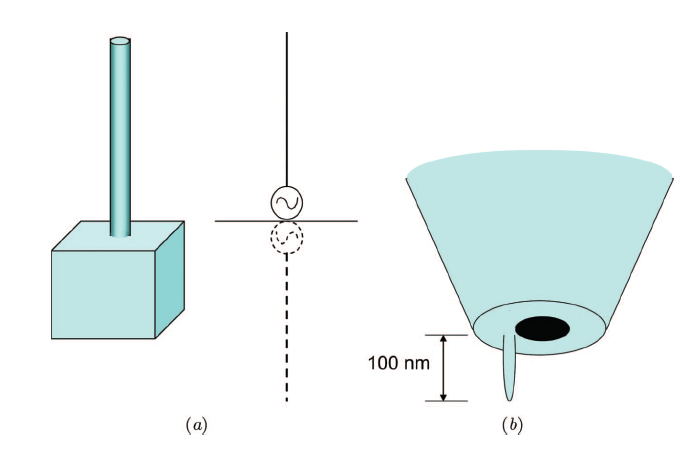
\includegraphics[width=0.35\textwidth]{optant1}
% \end{frame}

% \begin{frame}{Различие поведения металлов в радиодиапазоне и в оптике}
% \begin{itemize}
% \item В РД частота находится далеко от резонансной частоты плазменных колебаний электронов. Это означает, что отклик (воприимчивость и вытекающие из нее величины) почти стационарны и не зависят от частоты. В оптике зависимость от частоты носит ярко выраженный резонансный характер (это осложняет ситуацию, но и дает возможность получить высокую чувствительность и селективность).
% \item Скин-эффект в РД носит нормальный характер, т.к. длина свободного пробега электронов мала по сравнению с длиной волны: при частоте $\omega = 10$ МГц, толщина скин-слоя для меди $\Delta = 21$ мкм, т.е. \textcolor{red!50!black}{ $\Delta/\lambda \approx 10^{-6}$}. Металл отражает радиоволны почти полностью!

% \item В оптике скин-эффект носит аномальный характер.  Причием необходимо выделить три фактора. 1) Когда проникновение в металл определяется коллективными явлениями. Для описания скин-эффекта возникает необходимость учитывать еще одну величину $L_T=V_F/\omega$ , т.е. расстояние, которое проходит электрон за один период поля.
% \end{itemize}

% \end{frame}

% \begin{frame}{Три характерные длины}

% 1) Когда созданы условия для возбуждения плазмонов. Поперечный размер $SPP$ это $L_z=1/\Ima k_z$, где 
% \begin{equation*}
% k_z^2=\left(\frac{\omega}{c}\right)\frac{\epsilon_m^2}{\epsilon_m^2+\epsilon_d^2}
% \end{equation*} 
% Для золота $\lambda = 600$ нм, толщина $SPP$ $d_{SPP}=24$ нм, т.е. \textcolor{red!50!black}{$d_{SPP}/\lambda \approx 10^{-2}$}

% 2) $\lambda \approx \Delta$ (нижняя часть оптического спектра, ближе к ИК) имеет место аномальный скин-эффект (И.Н. Топтыгин "Современная электродинамика")
% \begin{equation*}
% \Delta \approx \left(\frac{c^2 p_F^2}{\omega N e^2}\right)^{1/3}
% \end{equation*}

% 3) $L_T <<\delta$ (высокая часть оптического спектра, ближе к УФ) мы как бы возращаемся в область нормального скин-эффекта, но роль $\lambda$ играет $L_T$
% \begin{equation*}
% \Delta \approx c \hbar/ \epsilon_F
% \end{equation*}
% для золота $\epsilon_F=5.53 eV$ имеем $\textcolor{red!50!black}{\Delta \approx 300\quad \text{нм, т.е.}\quad \Delta/\lambda\approx 1!}$


% \end{frame}


% \begin{frame}{Различие поведения металлов в радиодиапазоне и в оптике}
% \begin{itemize}
% \item В РД доминируют явления проводимости (разница составляет 4 порядка), а сами  метеллы в РД являются гораздо лучшими проводниками, чем в ОД.

% \item В ОД вместе с явлениями проводимости начинают играть роль эффекты поляризации. Т.е. когда мы воздействуем на металл с очень маленькой частотой, колебания электронного газа начинают отставать от вынуждающей силы, проявляя инерционность.

% \item Предыдущее означает, что наряду с током проводимости, значимую роль начинает играть ток смещения. С точки зрения радиоустройств это означает, что в РД диапазоне антенна имеет согласованную нагрузку со свободным пространством и может иметь длину кратную длине волны в свободном пространстве, а ОД - нет, т.о. мы не можем просто взять размер кратный длине волны.

% \item В приницпе в ОД антенны могут быть диэлектрическими, что невозможно представить себе в РД!

% \item И наконец, last but not least, в оптике возрастает поглощение, т.е. потери.
% \end{itemize}

% \end{frame}

% \begin{frame}{Литература}

% Наиболее значимые работы по оптическим антеннам:

% \begin{enumerate}

% \item Ю.С. Кившарь и др. \textbf{Оптические наноантенны}, Успехи физических наук, т.183, 2013.

% \item L. Novotny et al. \textbf{Optical antennas}, Advances in Optics and Photonics, 2009.

% \item M. B. Raschke \textbf{Antenna-load interactions at optical frequencies: impedance matching to quantum systems}, Nanotechnology, 2012.

% \item N. Engheta et al. \textbf{Theory, Modelling and Features of Optical Nanoantennas}, IEEE, 2013.

% \item D. W. Pohl et al. \textbf{Resonant optical Antennas}, Science, 2005.

% \item Q. Park \textbf{Optical antennas and plasmonics}, Contemporary Physics, 2009.
% \end{enumerate}
% \begin{center}
% 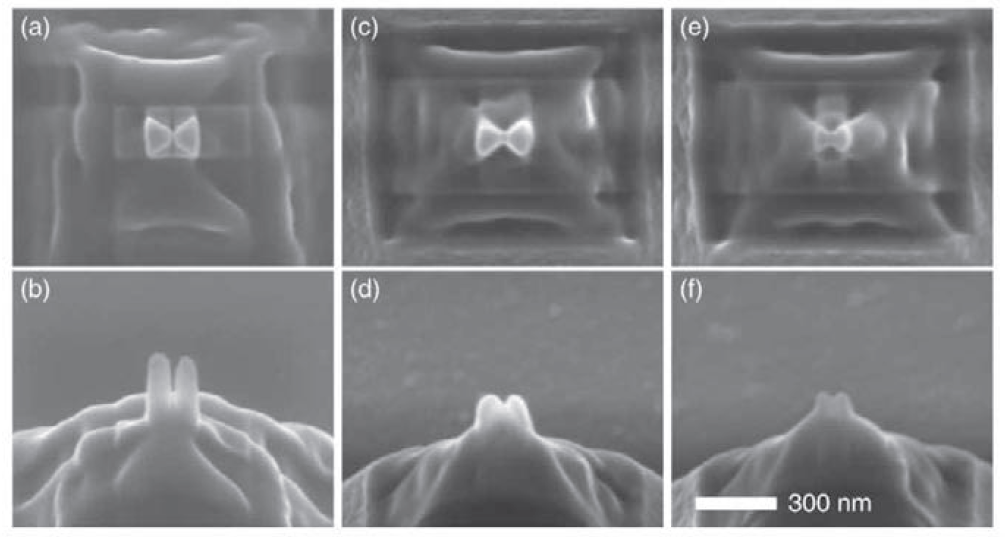
\includegraphics[width=0.4\textwidth]{optant2}
% \end{center}
% \end{frame}
% \begin{frame}{Масштабы величин}
% \begin{center}
% 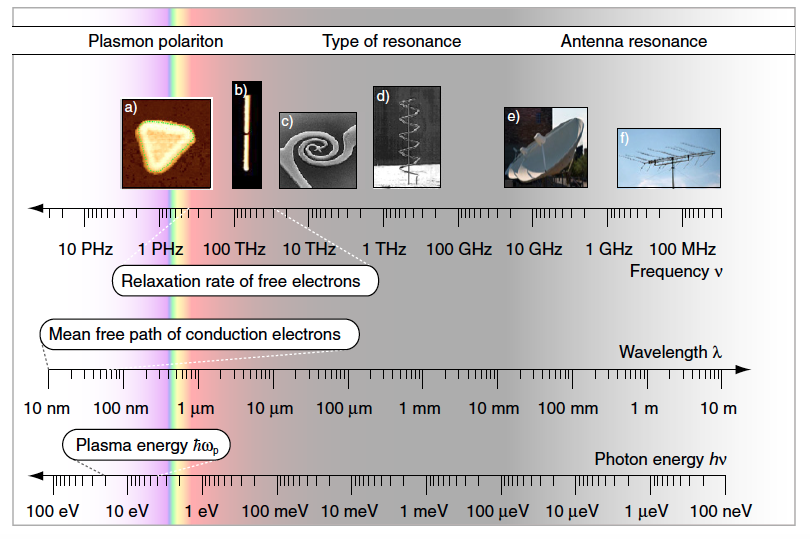
\includegraphics[width=0.9\textwidth]{optant50}

% Таким образом, следует признать, что механизм сгущения поля и его динамики во взаимодействии с окружающими объектами и средами в РД и ОД разные. Но эффективность в ОД не ниже, чем в РД, а порой даже выше. Чувствительность выше однозначно. 
% \end{center}

% \end{frame}

% \begin{frame}{Две схемы}
% \begin{columns}[c]
% \column{6.3cm}
% \begin{center}
% 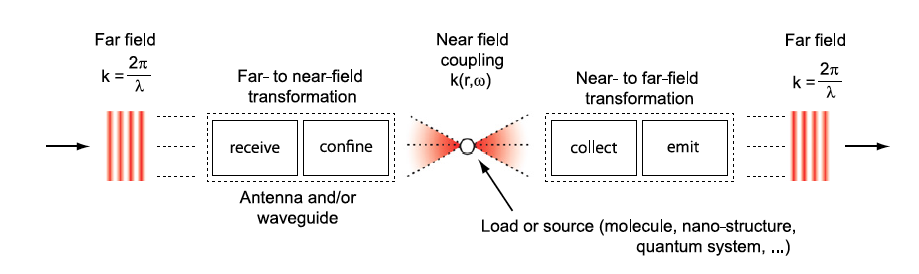
\includegraphics[width=\textwidth]{optant51}
% \end{center}

% {\small \textcolor{red!50!black}{Согласованная нагрузка (impedance matching):} если есть два двухполюсника, активный и пассивный, то наиболее эффективно активный двухполюсник будет передавать мощность пассивному (нагрузке, load) при равенстве импедансов. Простая механическая аналогия: если наливать воду через воронку в сосуд, то необходимо учиывать скорость прохождения воды через воронку, в противном случае часть воды выплеснется.}


% \column{6cm}
% \begin{center}
% 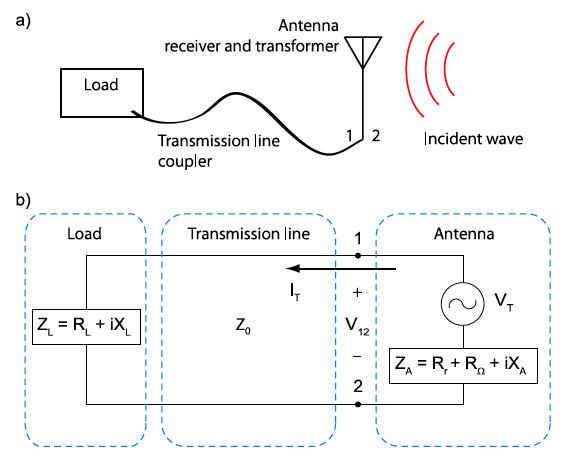
\includegraphics[width=0.8\textwidth]{optant52}
% \end{center}

% {\small В РД мы могли описать этот процесс посредством свойств активного и реактивного сопротивления. Хотя даже в случае идеального согласования лишь половина мощности оказывается в нагрузке, остальная диссипирует.}
% \end{columns}
 
%  В ОД мы вынуждены учитывать квантовую природу поглощения и испускания света. Для описания нам необходимо вводить локальную плотность электронных состояний (LDOS).
% \end{frame}

% \begin{frame}{Радиоантенна}
% \begin{columns}[c]
% \column{6.3cm}
% \begin{center}
% 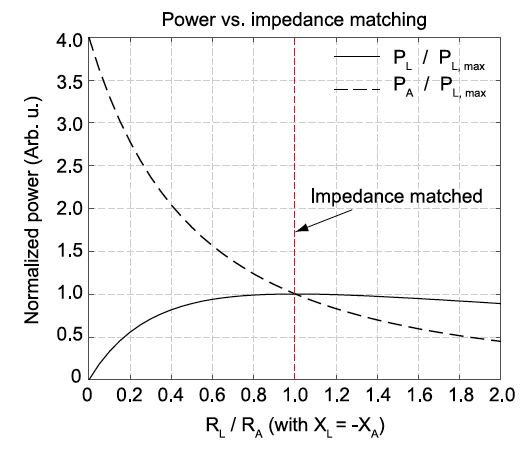
\includegraphics[width=0.8\textwidth]{optant53}
% \end{center}
% \column{6.3cm}
% \begin{center}
% 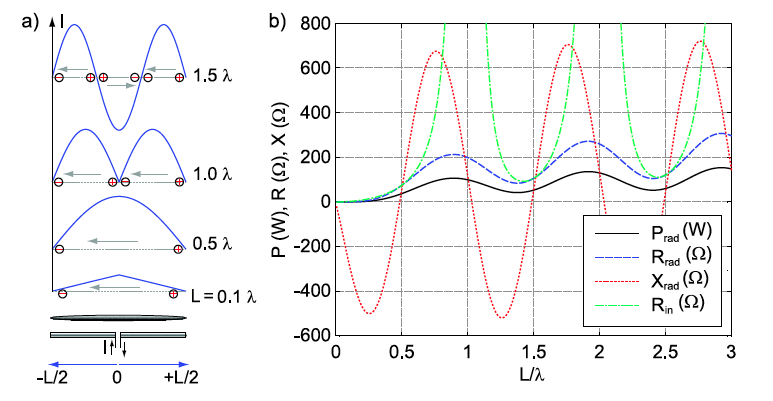
\includegraphics[width=\textwidth]{optant54}
% \end{center}
% \end{columns}

% {\small На основной волне и всех \textcolor{red!50!black}{нечетных гармониках} точки питания располагаются в пучности тока, и в антенне имеет место резонанс напряжения. При этом ее входное сопротивление невелико и равно сопротивлению потерь в цепи антенны. На всех \textcolor{red!50!black}{четных гармониках} точки, к которым подводится питание, оказываются расположенными в узлах тока, и в антенне имеет место резонанс тока. При этом ее входное сопротивление достигает весьма значительной величины.

% $\boxed{\text{Задача радиоантенны - доставить сигнал в дальнее поле с min искажениями.}}$}
% \end{frame}

% \begin{frame}{Металл в оптическом диапазоне}

% \begin{columns}[c]
% \column{6cm}
% \begin{center}
% 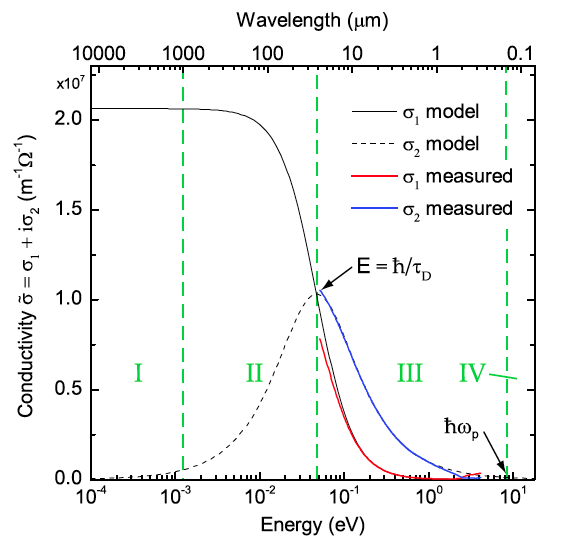
\includegraphics[width=0.7\textwidth]{optant56}
% \end{center}
% \textcolor{red!50!black}{Режимы:}

% \textcolor{red!50!black}{I} - режим Хагена-Рубенса, РД, ($\sigma_1<<\sigma_2$) электроны движутся практически в фазе с падающим полем.

% \textcolor{red!50!black}{II} - дальний ИК, переходный режим, нарастает релаксация $\gamma$, восп-ть $\epsilon(\omega) = 1-\frac{\omega_p^2}{\omega^2+\imath \gamma}$

% \column{6.2cm}
% \begin{center}
% 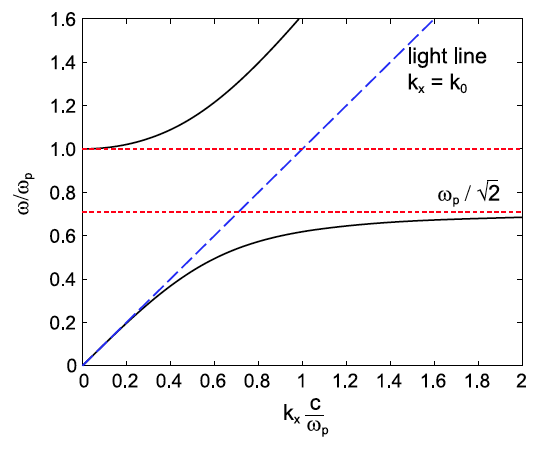
\includegraphics[width=0.7\textwidth]{optant57}
% \end{center}

% \textcolor{red!50!black}{III} - дальний - средний ИК, существенно возрастают омические потери, существенно фазовое запаздывание

% \textcolor{red!50!black}{IV} - область прозрачности за плазменной частотой.

% \end{columns}

% $\boxed{\text{Задача оптической антенны - доставить инорфмацию о ближнем поле.}}$

% \end{frame}

% \begin{frame}{Размер оптической антенны}

% Размер не буден кратен целому числу полуволн, как в РД.

% \begin{equation*}
% \boxed{\frac{m\lambda_{eff}}{2} = L(\lambda_{0})+2\psi(\lambda_0)}
% \end{equation*}

% \begin{center}
% 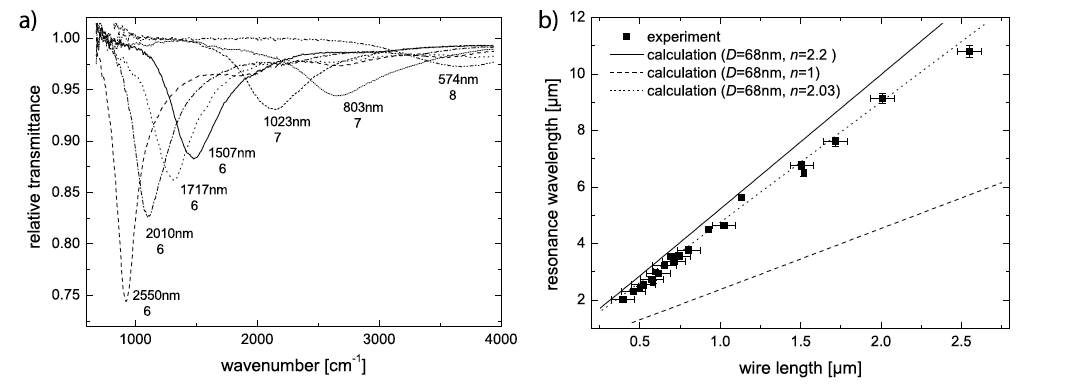
\includegraphics[width=0.8\textwidth]{optant60}

% 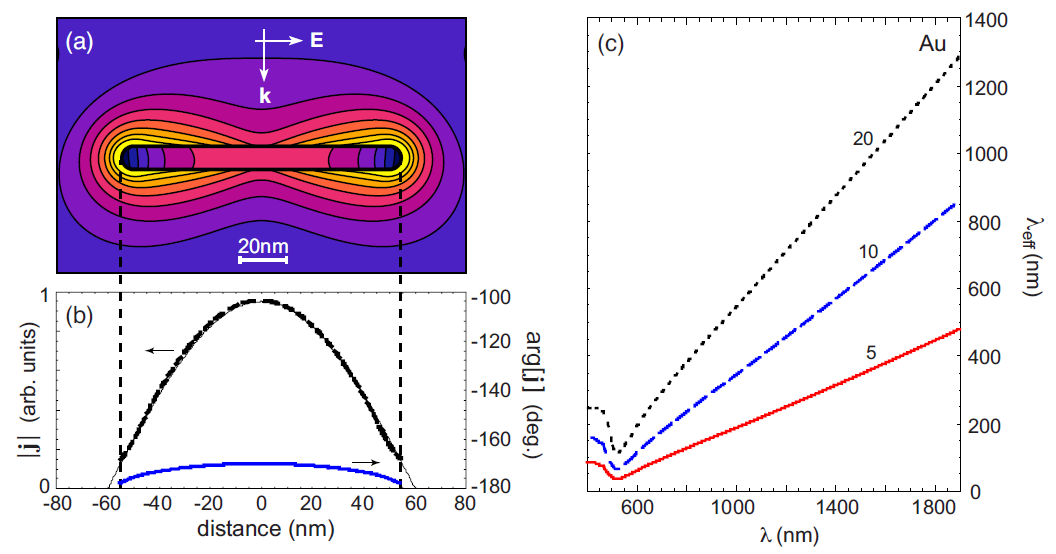
\includegraphics[width=0.55\textwidth]{optant_7}
% \end{center}
% \end{frame}

% \begin{frame}{Импеданс оптической антенны}

% Полная скорость релаксации двухуровневого квантового излучателя, находящегося в точке
% $\vec r_0$,

% \begin{equation*}
% \Gamma=\frac{\pi \omega}{3\hbar \epsilon_0}\left|\langle g| \hat{\vec p}| e \rangle\right|^2\rho_{p}(\vec r_0, \omega)
% \end{equation*}

% Здесь $\rho_{\vec p}$~--- парциальная ЛПС. Переходя к полной ЛПС путем усреднения по
% всем направлениям $\vec p$, получим
% \begin{equation*}
% \rho (\vec r_0, \omega) =\frac{2 \omega}{\pi c^2}\text{Im}\left\{\text{Tr}\left[\hat{\vec
% G}(\vec  r_0,\vec r_0;\omega_0)\right]\right\},
% \end{equation*}

% Функция Грина задается форм-фактором антенны и ее излучательными свойствами. Для
% свободного пространства без антенны, когда $\rho_{\vec p} = \omega^2/(\pi^2 c^3)$ для скорости релаксации получаем
% \begin{equation*}
% \Gamma_0=\omega^3\left|\langle g|\hat{\vec p}|e\rangle\right|^2/(3\pi^2
% \epsilon_0 \hbar c^3)
% \end{equation*}

% Пользуясь теоремой Пойтинга $P = \frac{1}{2} \int_V Re(\vec j* \times \vec E)dV$ и
% учитывая плотность тока в дипольном приближении $\vec j (\vec r) = - \imath \omega \vec p \delta(\vec r - \vec r_0)$,
% \end{frame}

% \begin{frame}{Импеданс оптической антенны}

% Получим выражение для мощности, рассеиваемого излучателем поля через ЛПС
% \begin{equation*}
% P =\frac{\pi \omega^2}{12 \epsilon_0}|\vec p|^2 \rho_{\vec p}^2(\vec r_0, \omega).
% \end{equation*}

% Вводя мощность рассеянного излучения в свободном пространстве как

% \begin{equation*}
% P_0 =\frac{\omega^4}{12 \pi \epsilon_0 c^3}|\vec p|^2
% \end{equation*}

% выразим ЛПС через нормированную мощность

% \begin{equation*}
% \rho_{\vec p}^2(\vec r_0, \omega) =\frac{\omega^2}{\pi^2 c^3}P/P_0
% \end{equation*}

% сравнивая выражение для $P$ с выражением для $\Gamma$, получим интересный результат:

% \begin{equation*} \frac{P}{\Gamma} = \frac{|\vec p|^2}{\left|\langle g| \hat{\vec p}| e
% \rangle\right|^2}\frac{\hbar \omega}{4}
% \end{equation*}
% \end{frame}


% \begin{frame}{Импеданс оптической антенны}

% Итак, импеданс оптической антенны может быть определен как $Re(Z)=P/I^2$, где мы
% вместо тока возьмем плотность тока $j \sim \imath \omega \vec p$

% \begin{equation*}
% Re(Z) = \frac{\pi}{12 \epsilon_0}\rho_{\vec p}^2(\vec r_0, \omega)
% \end{equation*}

% {\textcolor{red!50!black}{Свойства полученных результатов}
% \begin{enumerate}
% \item Мы должны различать скорость релаксации и скорость испускания фотона,
%     классический дипольный момент и дипольный момент перехода, первый простирается по $\omega$ от $-\infty$ до $+\infty$, а второй только от $0$ до $+\infty$, по свойству преобр. Фурье их разница в два раза

% \item ЛПС определяют, по сути, импеданс нашей оптической антенны

% \item  Импеданс антенны зависит как от расположения источника (или передатчика),
%     так и от ориентации его дипольного момента

% \item Мнимая часть импеданса даст нам энергию, сосредоточенную в ближнем поле
% \end{enumerate}


% \end{frame}
% \begin{frame}{Пример: антенна-наночастица}

% Рассмотрим в качестве антенны сферическую наночастицу

% \begin{center}
% 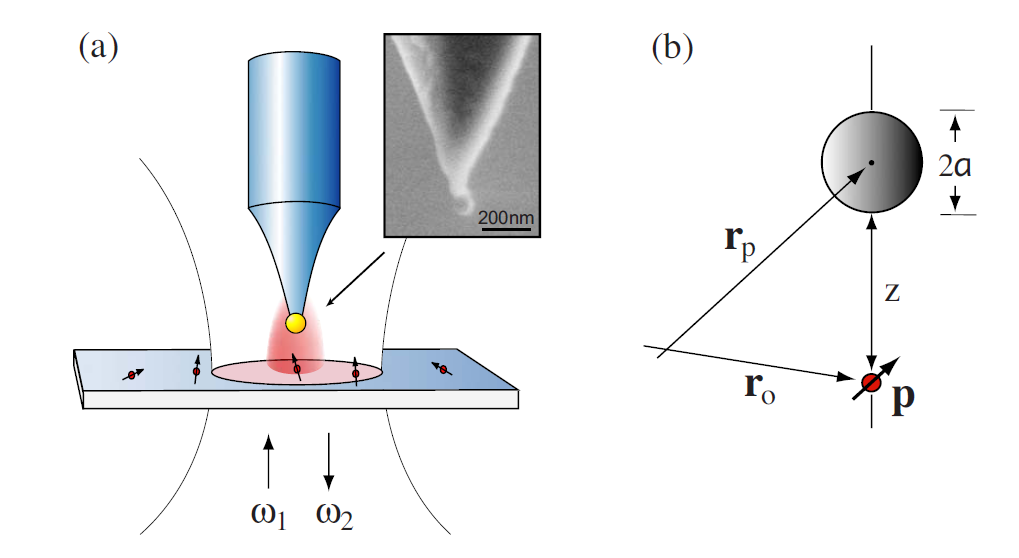
\includegraphics[width=7cm]{optant_5}
% \end{center}

%  Поляризуемость сферической частицы

% \begin{equation*}
% \alpha=4 \pi \epsilon_0 a^3 \frac{\epsilon(\omega)-1}{\epsilon(\omega)+2}
% \end{equation*}\documentclass[9pt, compress, xcolor=table]{beamer}


% \usetheme{m}

% \usepackage{amsmath,amssymb,amsthm}
% \usepackage{latexsym}
% \usepackage{booktabs}
% \usepackage[scale=2]{ccicons}
% \usepackage{minted}
% \usepackage[english, russian]{babel}
% \usepackage{graphicx}
% \usepackage{xcolor}
% \usepackage{tabu} % https://ru.sharelatex.com/learn/Tables
% \DeclareGraphicsExtensions{.pdf,.jpg,.png}
% \graphicspath{{../images/}{./images/}}

% \colorlet{Mycolor1}{green!50!blue!50!}
% \DeclareMathOperator{\Ima}{Im}
% \usemintedstyle{trac}

% \title{Физические принципы оптической микроскопии сверхвысокого разрешения}
% \subtitle{осенний семестр, 2015}
% \author{ассистент, к.ф.-м.н. Шутова О.А.}
% \institute{МГУ им. М.В. Ломоносова, физический факультет}

% \begin{document}

% \maketitle

% \plain{}{Лекция 6. Свойства оптических антенн}

% \begin{frame}{Идея лекции}


% Дальнейшее развитие ближнепольной микроскопии связано с таким фундаментальным понятием теории электромагнетизма как \textcolor{red!50!black}{антенна}. 

% \textcolor{red!50!black}{Антенна} - это такое устройство, которое может \textcolor{red!50!black}{эффективно} преобразовывать э.м. энергию в распространяющееся э.м. излучение и наоборот. Изначально это понятие возникло в области длинных волн (радиодиапазон). Интересно, что в [2] (см. ниже) указывается на общность корней в слове \textbf{антенна} и \textbf{тянуть} через общий корень в санскрите $tan$. 

% Переход в оптический диапазон, во многом столь же исторически значимый, как переход от мазеров к лазерам, НЕ может быть связан с простым переносом понятий из области радиоантенн в область оптических антенн по причине того, что \textbf{поведение металлов в области длинных волн и коротких носит существенно разный характер}.

% \centering
% 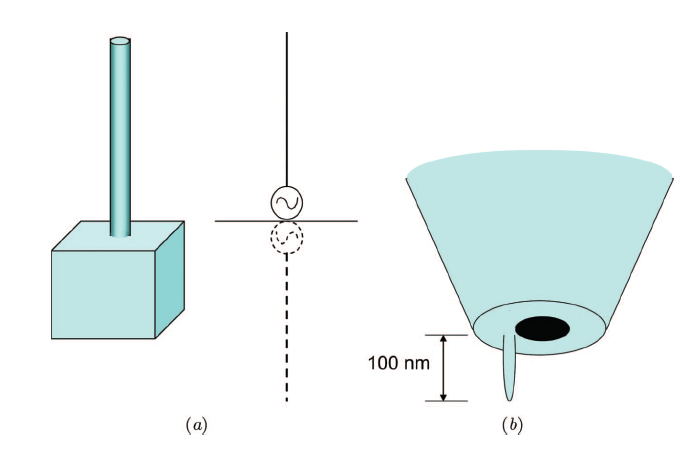
\includegraphics[width=0.35\textwidth]{optant1}
% \end{frame}

% \begin{frame}{Различие поведения металлов в радиодиапазоне и в оптике}
% \begin{itemize}
% \item В РД частота находится далеко от резонансной частоты плазменных колебаний электронов. Это означает, что отклик (воприимчивость и вытекающие из нее величины) почти стационарны и не зависят от частоты. В оптике зависимость от частоты носит ярко выраженный резонансный характер (это осложняет ситуацию, но и дает возможность получить высокую чувствительность и селективность).
% \item Скин-эффект в РД носит нормальный характер, т.к. длина свободного пробега электронов мала по сравнению с длиной волны: при частоте $\omega = 10$ МГц, толщина скин-слоя для меди $\Delta = 21$ мкм, т.е. \textcolor{red!50!black}{ $\Delta/\lambda \approx 10^{-6}$}. Металл отражает радиоволны почти полностью!

% \item В оптике скин-эффект носит аномальный характер.  Причием необходимо выделить три фактора. 1) Когда проникновение в металл определяется коллективными явлениями. Для описания скин-эффекта возникает необходимость учитывать еще одну величину $L_T=V_F/\omega$ , т.е. расстояние, которое проходит электрон за один период поля.
% \end{itemize}

% \end{frame}

% \begin{frame}{Три характерные длины}

% 1) Когда созданы условия для возбуждения плазмонов. Поперечный размер $SPP$ это $L_z=1/\Ima k_z$, где 
% \begin{equation*}
% k_z^2=\left(\frac{\omega}{c}\right)\frac{\epsilon_m^2}{\epsilon_m^2+\epsilon_d^2}
% \end{equation*} 
% Для золота $\lambda = 600$ нм, толщина $SPP$ $d_{SPP}=24$ нм, т.е. \textcolor{red!50!black}{$d_{SPP}/\lambda \approx 10^{-2}$}

% 2) $\lambda \approx \Delta$ (нижняя часть оптического спектра, ближе к ИК) имеет место аномальный скин-эффект (И.Н. Топтыгин "Современная электродинамика")
% \begin{equation*}
% \Delta \approx \left(\frac{c^2 p_F^2}{\omega N e^2}\right)^{1/3}
% \end{equation*}

% 3) $L_T <<\delta$ (высокая часть оптического спектра, ближе к УФ) мы как бы возращаемся в область нормального скин-эффекта, но роль $\lambda$ играет $L_T$
% \begin{equation*}
% \Delta \approx c \hbar/ \epsilon_F
% \end{equation*}
% для золота $\epsilon_F=5.53 eV$ имеем $\textcolor{red!50!black}{\Delta \approx 300\quad \text{нм, т.е.}\quad \Delta/\lambda\approx 1!}$


% \end{frame}


% \begin{frame}{Различие поведения металлов в радиодиапазоне и в оптике}
% \begin{itemize}
% \item В РД доминируют явления проводимости (разница составляет 4 порядка), а сами  метеллы в РД являются гораздо лучшими проводниками, чем в ОД.

% \item В ОД вместе с явлениями проводимости начинают играть роль эффекты поляризации. Т.е. когда мы воздействуем на металл с очень маленькой частотой, колебания электронного газа начинают отставать от вынуждающей силы, проявляя инерционность.

% \item Предыдущее означает, что наряду с током проводимости, значимую роль начинает играть ток смещения. С точки зрения радиоустройств это означает, что в РД диапазоне антенна имеет согласованную нагрузку со свободным пространством и может иметь длину кратную длине волны в свободном пространстве, а ОД - нет, т.о. мы не можем просто взять размер кратный длине волны.

% \item В приницпе в ОД антенны могут быть диэлектрическими, что невозможно представить себе в РД!

% \item И наконец, last but not least, в оптике возрастает поглощение, т.е. потери.
% \end{itemize}

% \end{frame}

% \begin{frame}{Литература}

% Наиболее значимые работы по оптическим антеннам:

% \begin{enumerate}

% \item Ю.С. Кившарь и др. \textbf{Оптические наноантенны}, Успехи физических наук, т.183, 2013.

% \item L. Novotny et al. \textbf{Optical antennas}, Advances in Optics and Photonics, 2009.

% \item M. B. Raschke \textbf{Antenna-load interactions at optical frequencies: impedance matching to quantum systems}, Nanotechnology, 2012.

% \item N. Engheta et al. \textbf{Theory, Modelling and Features of Optical Nanoantennas}, IEEE, 2013.

% \item D. W. Pohl et al. \textbf{Resonant optical Antennas}, Science, 2005.

% \item Q. Park \textbf{Optical antennas and plasmonics}, Contemporary Physics, 2009.
% \end{enumerate}
% \begin{center}
% 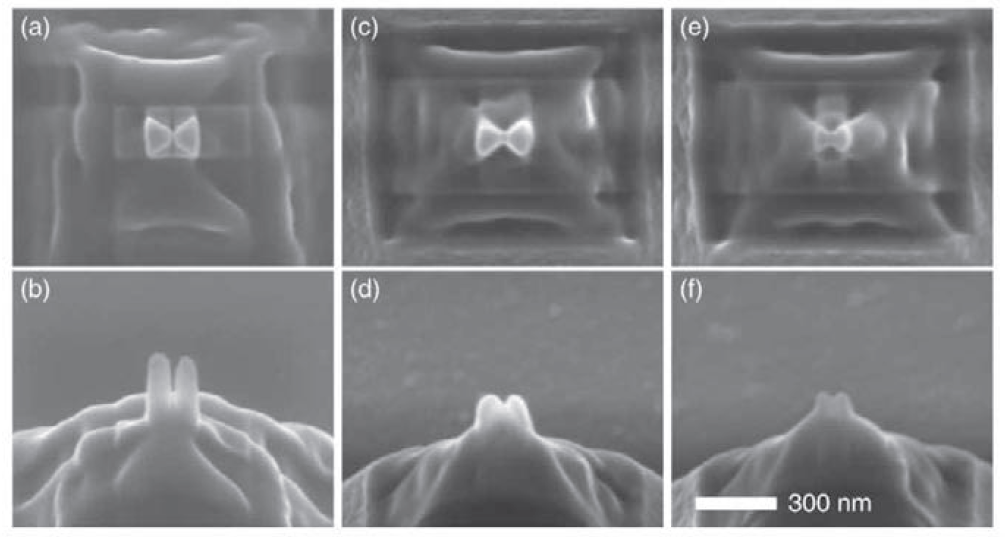
\includegraphics[width=0.4\textwidth]{optant2}
% \end{center}
% \end{frame}
% \begin{frame}{Масштабы величин}
% \begin{center}
% 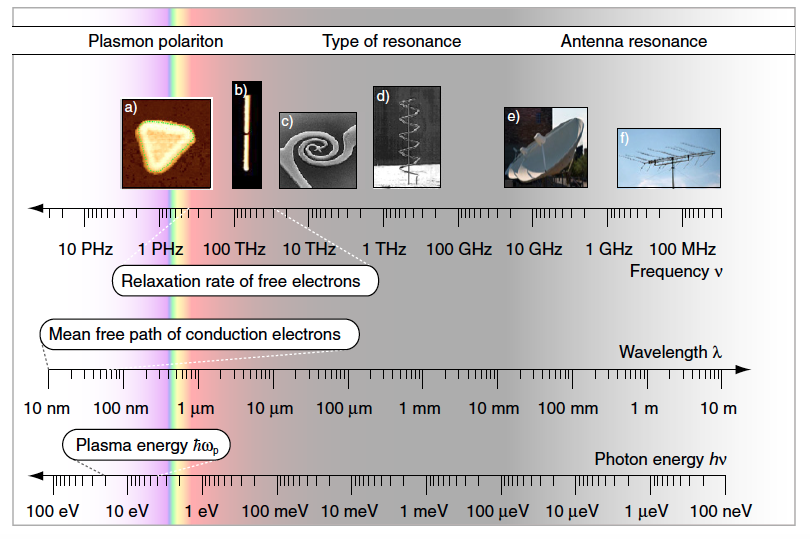
\includegraphics[width=0.9\textwidth]{optant50}

% Таким образом, следует признать, что механизм сгущения поля и его динамики во взаимодействии с окружающими объектами и средами в РД и ОД разные. Но эффективность в ОД не ниже, чем в РД, а порой даже выше. Чувствительность выше однозначно. 
% \end{center}

% \end{frame}

% \begin{frame}{Две схемы}
% \begin{columns}[c]
% \column{6.3cm}
% \begin{center}
% 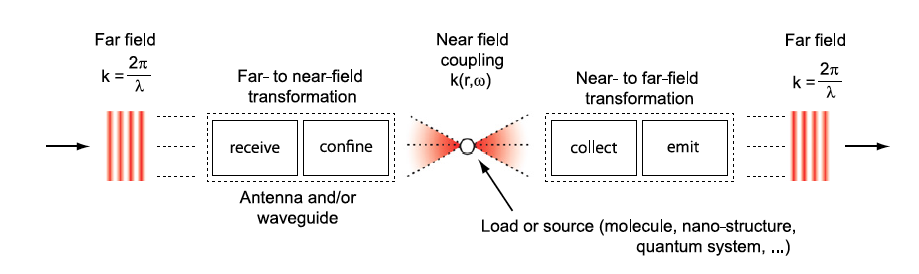
\includegraphics[width=\textwidth]{optant51}
% \end{center}

% {\small \textcolor{red!50!black}{Согласованная нагрузка (impedance matching):} если есть два двухполюсника, активный и пассивный, то наиболее эффективно активный двухполюсник будет передавать мощность пассивному (нагрузке, load) при равенстве импедансов. Простая механическая аналогия: если наливать воду через воронку в сосуд, то необходимо учиывать скорость прохождения воды через воронку, в противном случае часть воды выплеснется.}


% \column{6cm}
% \begin{center}
% 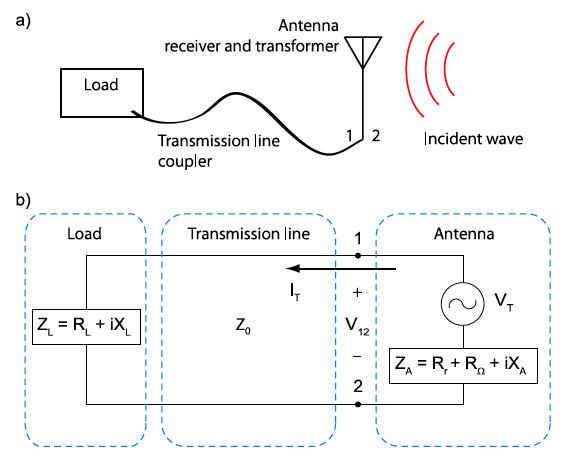
\includegraphics[width=0.8\textwidth]{optant52}
% \end{center}

% {\small В РД мы могли описать этот процесс посредством свойств активного и реактивного сопротивления. Хотя даже в случае идеального согласования лишь половина мощности оказывается в нагрузке, остальная диссипирует.}
% \end{columns}
 
%  В ОД мы вынуждены учитывать квантовую природу поглощения и испускания света. Для описания нам необходимо вводить локальную плотность электронных состояний (LDOS).
% \end{frame}

% \begin{frame}{Радиоантенна}
% \begin{columns}[c]
% \column{6.3cm}
% \begin{center}
% 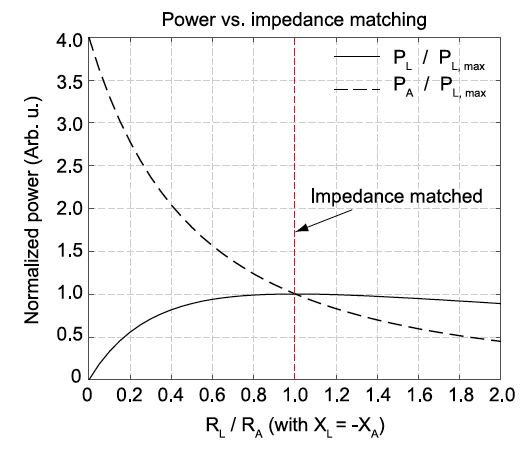
\includegraphics[width=0.8\textwidth]{optant53}
% \end{center}
% \column{6.3cm}
% \begin{center}
% 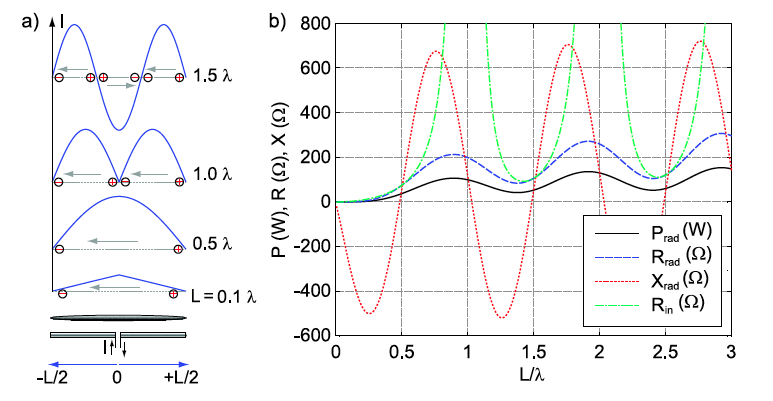
\includegraphics[width=\textwidth]{optant54}
% \end{center}
% \end{columns}

% {\small На основной волне и всех \textcolor{red!50!black}{нечетных гармониках} точки питания располагаются в пучности тока, и в антенне имеет место резонанс напряжения. При этом ее входное сопротивление невелико и равно сопротивлению потерь в цепи антенны. На всех \textcolor{red!50!black}{четных гармониках} точки, к которым подводится питание, оказываются расположенными в узлах тока, и в антенне имеет место резонанс тока. При этом ее входное сопротивление достигает весьма значительной величины.

% $\boxed{\text{Задача радиоантенны - доставить сигнал в дальнее поле с min искажениями.}}$}
% \end{frame}

% \begin{frame}{Металл в оптическом диапазоне}

% \begin{columns}[c]
% \column{6cm}
% \begin{center}
% 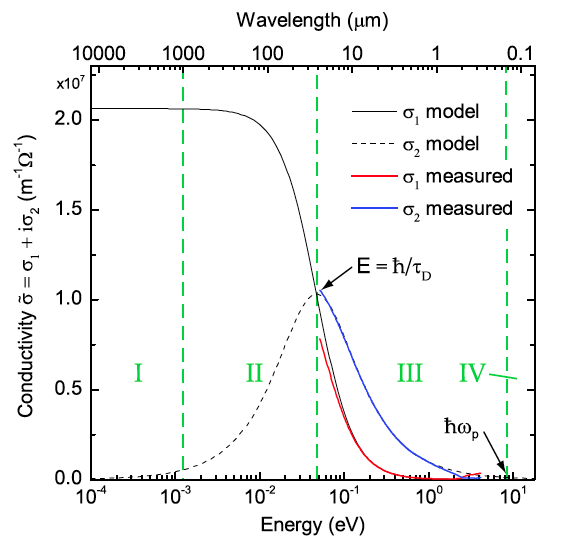
\includegraphics[width=0.7\textwidth]{optant56}
% \end{center}
% \textcolor{red!50!black}{Режимы:}

% \textcolor{red!50!black}{I} - режим Хагена-Рубенса, РД, ($\sigma_1<<\sigma_2$) электроны движутся практически в фазе с падающим полем.

% \textcolor{red!50!black}{II} - дальний ИК, переходный режим, нарастает релаксация $\gamma$, восп-ть $\epsilon(\omega) = 1-\frac{\omega_p^2}{\omega^2+\imath \gamma}$

% \column{6.2cm}
% \begin{center}
% 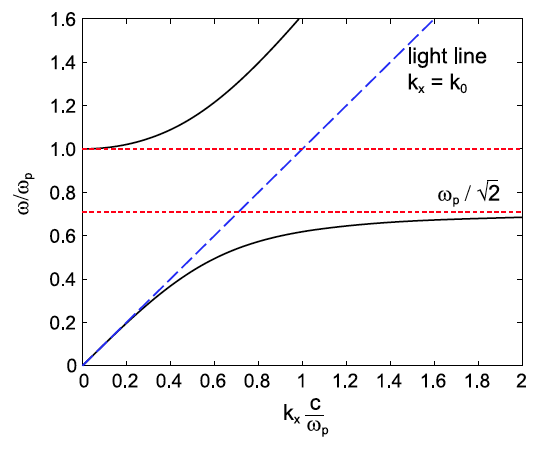
\includegraphics[width=0.7\textwidth]{optant57}
% \end{center}

% \textcolor{red!50!black}{III} - дальний - средний ИК, существенно возрастают омические потери, существенно фазовое запаздывание

% \textcolor{red!50!black}{IV} - область прозрачности за плазменной частотой.

% \end{columns}

% $\boxed{\text{Задача оптической антенны - доставить инорфмацию о ближнем поле.}}$

% \end{frame}

% % \begin{frame}{Размер оптической антенны}

% % Размер не буден кратен целому числу полуволн, как в РД.

% % \begin{equation*}
% % \boxed{\frac{m\lambda_{eff}}{2} = L(\lambda_{0})+2\psi(\lambda_0)}
% % \end{equation*}

% % \begin{center}
% % 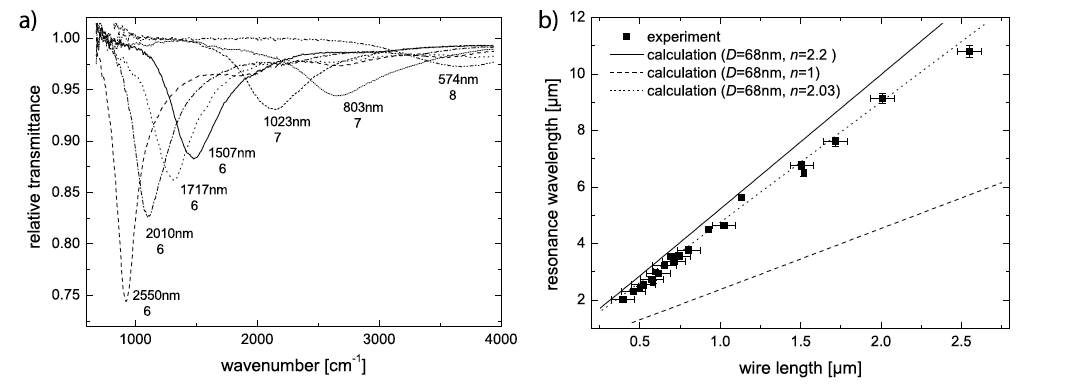
\includegraphics[width=0.8\textwidth]{optant60}

% % 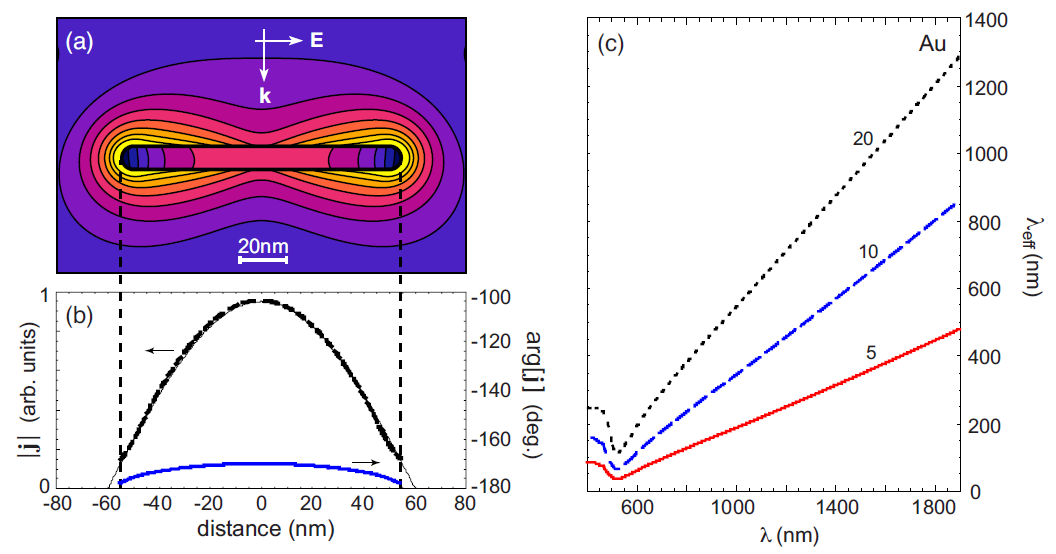
\includegraphics[width=0.55\textwidth]{optant_7}
% % \end{center}
% % \end{frame}

% % \begin{frame}{Импеданс оптической антенны}

% % Полная скорость релаксации двухуровневого квантового излучателя, находящегося в точке
% % $\vec r_0$,

% % \begin{equation*}
% % \Gamma=\frac{\pi \omega}{3\hbar \epsilon_0}\left|\langle g| \hat{\vec p}| e \rangle\right|^2\rho_{p}(\vec r_0, \omega)
% % \end{equation*}

% % Здесь $\rho_{\vec p}$~--- парциальная ЛПС. Переходя к полной ЛПС путем усреднения по
% % всем направлениям $\vec p$, получим
% % \begin{equation*}
% % \rho (\vec r_0, \omega) =\frac{2 \omega}{\pi c^2}\text{Im}\left\{\text{Tr}\left[\hat{\vec
% % G}(\vec  r_0,\vec r_0;\omega_0)\right]\right\},
% % \end{equation*}

% % Функция Грина задается форм-фактором антенны и ее излучательными свойствами. Для
% % свободного пространства без антенны, когда $\rho_{\vec p} = \omega^2/(\pi^2 c^3)$ для скорости релаксации получаем
% % \begin{equation*}
% % \Gamma_0=\omega^3\left|\langle g|\hat{\vec p}|e\rangle\right|^2/(3\pi^2
% % \epsilon_0 \hbar c^3)
% % \end{equation*}

% % По теореме Пойтинга $P = \frac{1}{2} \int_V Re(\vec j \times \vec E)dV$ и
% % учитывая плотность тока в дипольном приближении $\vec j (\vec r) = - \imath \omega \vec p \delta(\vec r - \vec r_0)$.
% % \end{frame}

% % \begin{frame}{Импеданс оптической антенны}

% % Получим выражение для мощности, рассеиваемого излучателем поля, через ЛПС
% % \begin{equation*}
% % P =\frac{\pi \omega^2}{12 \epsilon_0}|\vec p|^2 \rho_{\vec p}^2(\vec r_0, \omega).
% % \end{equation*}

% % Вводя мощность рассеянного излучения в свободном пространстве как

% % \begin{equation*}
% % P_0 =\frac{\omega^4}{12 \pi \epsilon_0 c^3}|\vec p|^2
% % \end{equation*}

% % выразим ЛПС через нормированную мощность

% % \begin{equation*}
% % \rho_{\vec p}^2(\vec r_0, \omega) =\frac{\omega^2}{\pi^2 c^3}P/P_0
% % \end{equation*}

% % сравнивая выражение для $P$ с выражением для $\Gamma$, получим интересный результат:

% % \begin{equation*} \frac{P}{\Gamma} = \frac{|\vec p|^2}{\left|\langle g| \hat{\vec p}| e
% % \rangle\right|^2}\frac{\hbar \omega}{4}
% % \end{equation*}
% % \end{frame}


% % \begin{frame}{Импеданс оптической антенны}

% % Итак, импеданс оптической антенны может быть определен как $Re(Z)=P/I^2$, где мы
% % вместо тока возьмем плотность тока $j\sim \imath \omega \vec p$

% % \begin{equation*}
% % Re(Z) = \frac{\pi}{12 \epsilon_0}\rho_{\vec p}^2(\vec r_0, \omega)
% % \end{equation*}

% % \textcolor{red!50!black}{Свойства полученных результатов:}
% % \begin{enumerate}
% % \item Мы должны различать скорость релаксации и скорость испускания фотона,
% %     классический дипольный момент и дипольный момент перехода, первый простирается по $\omega$ от $-\infty$ до $+\infty$, а второй только от $0$ до $+\infty$, по свойству преобр. Фурье их разница в два раза

% % \item ЛПС определяют, по сути, импеданс нашей оптической антенны

% % \item  Импеданс антенны зависит как от расположения источника (или передатчика),
% %     так и от ориентации его дипольного момента

% % \item Мнимая часть импеданса даст нам энергию, сосредоточенную в ближнем поле
% % \end{enumerate}


% % \end{frame}


% % \begin{frame}{Пример: антенна-наночастица}

% % Рассмотрим в качестве антенны сферическую наночастицу

% % \begin{center}
% % 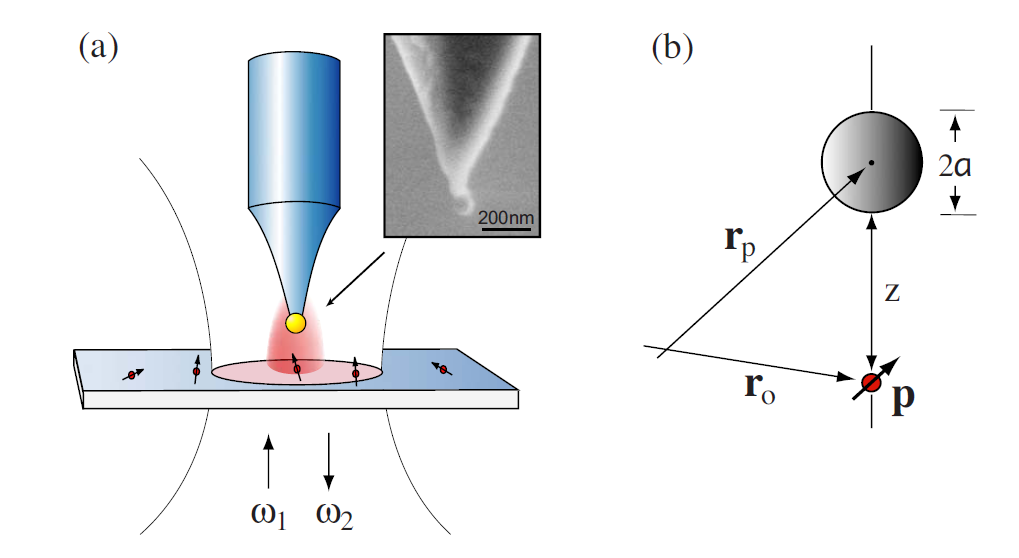
\includegraphics[width=7cm]{optant_5}
% % \end{center}

% %  Поляризуемость сферической частицы

% % \begin{equation*}
% % \alpha=4 \pi \epsilon_0 a^3 \frac{\epsilon(\omega)-1}{\epsilon(\omega)+2}
% % \end{equation*}

% % при $\epsilon(\omega)=-2$ имеем хорошо известное условие плазмонного резонанса на
% % сфере

% % \end{frame}


% % \begin{frame}{Пример: антенна-наночастица}
% % Поле может быть получено из тензорной функции Грина
% % \begin{equation*}
% % \vec E = \left[\overleftrightarrow I + \frac{k^2}{\epsilon_0}\alpha(\omega)
% % \overleftrightarrow G(\vec r_0, \vec r_0,\omega)\right] = \left[1+ 2 \overleftrightarrow\alpha(\omega)
% % \frac{a^3}{(a+z)^3}\right]\vec E_0
% % \end{equation*}}
% % {\scriptsize ЛПС:\begin{equation*} \rho_z(z)= \frac{\omega^2}{\pi^2 c^3}\left[\left|1+2
% % \frac{\epsilon(\omega)-1}{\epsilon(\omega)+2}\frac{a^3}{(a+z)^3}\right|^2+ \frac{3}{4} \Ima
% % \frac{\epsilon(\omega)-1}{\epsilon(\omega)+1}\frac{1}{(kz)^3}\right]
% % \end{equation*}

% % чем меньше собственный квантовый выход молекулы $\eta_i$, тем большее усиление может
% % быть получено
% % \begin{center}
% % 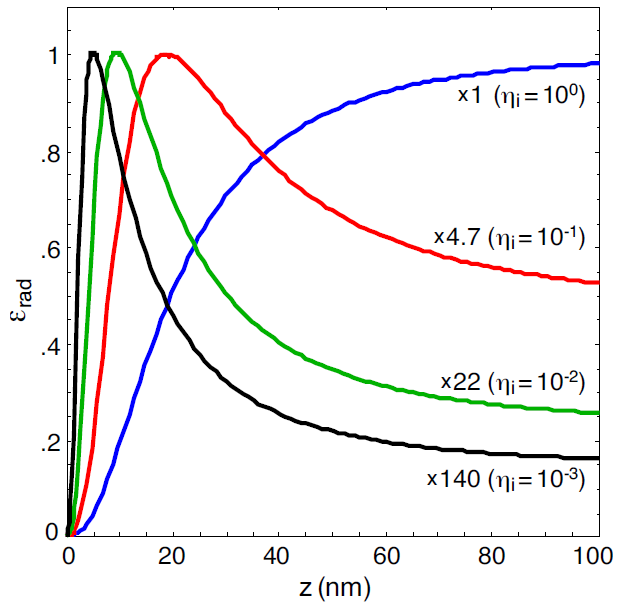
\includegraphics[width=4cm]{optant_6}
% % \end{center}

% % \end{frame}


% \end{document}

% \begin{frame}{}
% \begin{columns}[c]
% \column{6.5cm}
% \column{6cm}
% \begin{center}
% \includegraphics[width=0.9\textwidth]{}
% \end{center}
% \end{columns}
% \end{frame}


